\chapter{Einleitung}
\label{chap:einleitung}

In dieser Arbeit soll, mit Hilfe einer Simulation, untersucht werden, wie gut sich Kameras bei der Standortbestimmung in mobilen Roboter einsetzen lassen. Anlass dieser Arbeit war eine Anfrage der K�nstlergruppe \ac{BBM}, die schon bei mehreren Performances\footnote{unter Anderem:
  
  2000 Themenpark "Wissen" der Expo 2000 Hannover
  
  2010 Joybots  in der BMW-Welt 
  
  2012 EPKOT Experimental Prototype Killers of Tomorrow , Hannover
  
  siehe auch \url{ http://www.bbm.cfnt3.de}} mobile Roboter eingesetzt hat. Diese fahren zum Teil in einer Choreografie �ber die B�hne. Um sie dabei eine vorgegebene Figur fahren zu lassen, muss der Steuerung bekannt sein, wo sich ein Roboter auf der B�hne aufh�lt. Eine solche Lokalisation war in der Vergangenheit f�r BBM sehr aufwendig. Aus diesem Grund interessierte sie sich f�r eine Lokalisierungsl�sung welche m�glichst ohne weitere Spezialhardware und geringem Installationsaufwand vor Ort auskommt. Der Ansatz der daraus entstand war: die Kameras, die bereits an jedem der Roboter verbaut waren, zu nutzen um markante Muster in der B�hneninstallation zu erkennen. Zusammen mit Messungen der Odometrie, sie beschreibt wie die R�der eines Roboters sich bei Bewegung drehen, soll die Position und Orientierung berechnet werden. Ein Partikelfilter w�re als Zustandssch�tzer zu verwendet. Zu der B�hneninstallation geh�ren gro�e Lichtw�nde, zu sehen auf Abbildung \ref{fig:RobotAndGuests} und \ref{fig:RobotAndLightwall}. Auf diesen Lichtw�nden k�nnte ein hell/dunkel Bit-Muster angezeigt werden das es mit Hilfe geeigneter Bildverarbeitungsalgorithmen und mit den Kameras zu erkennen gilt.

  \begin{figure}[p]
    \centering
    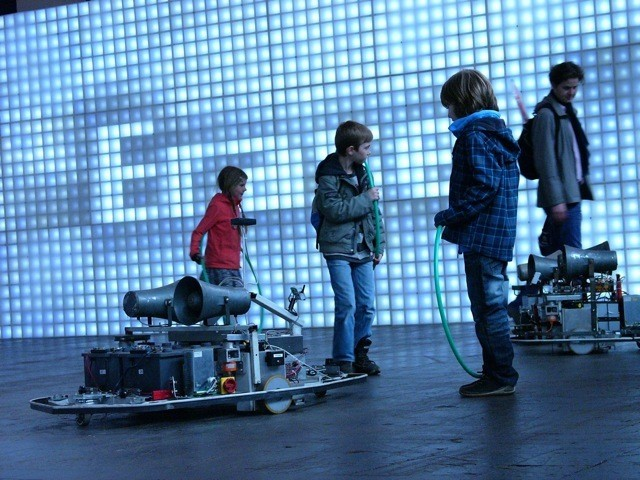
\includegraphics[width=\textwidth]{chapter1/roboterAndLightwallOnEPKOT2.png}
    \caption[Roboter und Besucher auf der EPKOT]{Roboter und Besucher auf der EPKOT Quelle: http://www.bbm.cfnt3.de}
    \label{fig:RobotAndGuests}
    \bigskip 
    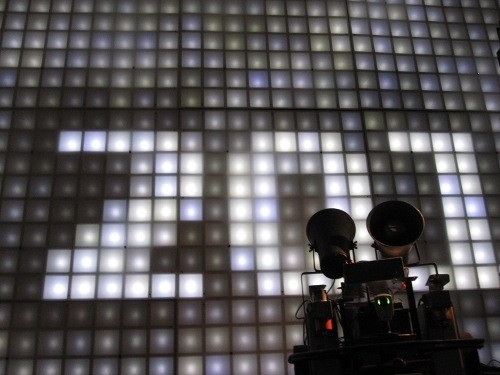
\includegraphics[width=\textwidth]{chapter1/roboterAndLightwallOnEPKOT.png}
    \caption[Roboter vor Lichtwand auf der EPKOT]{Roboter vor Lichtwand auf der EPKOT Quelle: http://www.bbm.cfnt3.de}
    \label{fig:RobotAndLightwall}
  \end{figure}
  
  \section{Ziel und Aufgabenstellung der Arbeit}
Im Rahmen dieser Arbeit soll eine Simulationsumgebung mit Hilfe geeigneter 3D-Visualisierungs Bibliotheken erstellt werden. Diese soll in der Lange sein eine 3D-Szene der B�hne zu simulieren und Kamerabilder sowie Odometrie-Daten einer Roboterfahrt zu erzeugen. Des weiten soll ein Lokalisationsalgorithmus entwickelt werden, der auf Grundlage dieser Daten die Position und Orientierung des Roboters auf der B�hne sch�tzen kann. Anschlie�end soll die Qualit�t dieser gesch�tzten Position beurteilt werden und m�gliche Fehlerquellen diskutiert werden.

  \section{Gliederung}
Die Arbeit wird im folgenden Kapitel eine kurze �bersicht g�ngiger Lokalisationsverfahren sowie deren Vor- und Nachteile geben. Au�erdem wird in die Grundlagen eingef�hrt, welche zum Verst�ndnis der folgenden Kapitel notwendig sind. Das Kapitel \textit{\nameref{chap:lokalisierungmittelsbildverarbeitung}} beschreibt wie die Methoden aus den Grundlagen an das gestellte Problem angepasst wurden und wie das vorgestellte Verfahren funktioniert. Anschlie�end wird die Simulations- und Lokalisationssoftware vorgestellt, deren Implementation erkl�rt und begr�ndet. Insbesondere wird darauf eingegangen, wie realistisch die Simulation ist. In Kapitel \ref{chap:versuche} beginnt die Beschreibung verschiedener Versuche die zum Beurteilen der Lokalisationsergebnisse durchgef�hrt wurden. Ergebnispr�sentation und Diskussion erfolgen jeweils im Anschluss der Beschreibungen. Abschlie�end wird ein Ausblick zur m�glichen Anwendung dieses Verfahrens gegeben, sowie m�gliche Fehlerquellen und Probleme dabei. Im letzten Kapitel wird ein Fazit zu den Erkenntnissen dieser Arbeit gezogen.
